\documentclass[tikz,border=15pt]{standalone}
\usepackage{amsmath,amssymb}
\usetikzlibrary{calc}

\begin{document}
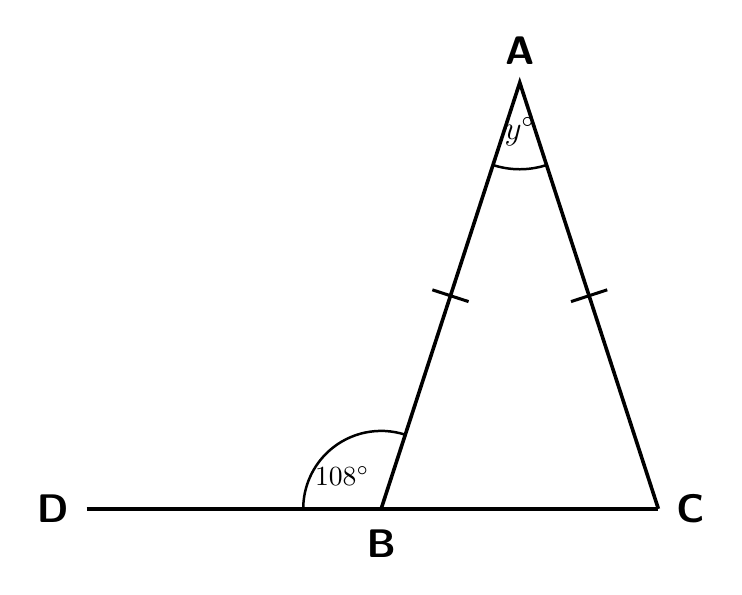
\begin{tikzpicture}[scale=1.1]
    % Isosceles triangle with base angles 72 deg, apex angle 36 deg
    % Base BC = 3.2 cm, B at (0,0), C at (3.2, 0)
    % A at (1.6, 1.6 * tan(72 deg)) = (1.6, 4.92)
    \coordinate (D) at (-3.4, 0);
    \coordinate (B) at (0, 0);
    \coordinate (C) at (3.2, 0);
    \coordinate (A) at (1.6, 4.92);
    
    % Draw extended baseline DBC
    \draw[line width=1.3pt] (D) -- (C);
    
    % Draw triangle sides AB and AC
    \draw[line width=1.3pt] (B) -- (A) -- (C);
    
    % Congruence tick marks on AB and AC
    \coordinate (MidAB) at ($(A)!0.5!(B)$);
    \coordinate (MidAC) at ($(A)!0.5!(C)$);
    \draw[line width=1.1pt] ($(MidAB) + ({72+90}:0.22)$) -- ($(MidAB) + ({72-90}:0.22)$);
    \draw[line width=1.1pt] ($(MidAC) + ({108+90}:0.22)$) -- ($(MidAC) + ({108-90}:0.22)$);
    
    % Exterior angle 108 deg at B (from 72 to 180)
    \draw[line width=0.9pt] ($(B) + (72:0.9)$) arc (72:180:0.9);
    \node[font=\bfseries] at (-0.45, 0.38) {$108^\circ$};
    
    % Apex angle y deg at A (from 252 to 288, span 36 deg)
    \draw[line width=0.9pt] ($(A) + (252:1.0)$) arc (252:288:1.0);
    \node[font=\large\bfseries] at (1.6, 4.35) {$y^\circ$};
    
    % Vertices labels in bold sans-serif
    \node[above=3pt, font=\Large\sffamily\bfseries] at (A) {A};
    \node[below=4pt, font=\Large\sffamily\bfseries] at (B) {B};
    \node[right=3pt, font=\Large\sffamily\bfseries] at (C) {C};
    \node[left=3pt, font=\Large\sffamily\bfseries] at (D) {D};
    
\end{tikzpicture}
\end{document}
